%--------------------------------------------------------------------
%
%Mustervorlage fuer eine Aufgabe
%
%--------------------------------------------------------------------
%
%Ueberschreiben der automatisch erzeugten Aufgabennummer
%Die folgende Aufgabennummer ergibt sich aus dem Stand des
%Z�hlers + 1
%\setcounter{chapter}{0}
%
\chapter{Blockschaltbild}\label{ex:blockschaltbild}
%
%Teilaufgabe 1
%
\section{}\label{sec:blockschaltbild}
%
Nachfolgend wird das Blockschaltbild des Regelkreises dargestellt (Abb. \ref{pic:blockschaltbild}):

\begin{figure}[htb]
%
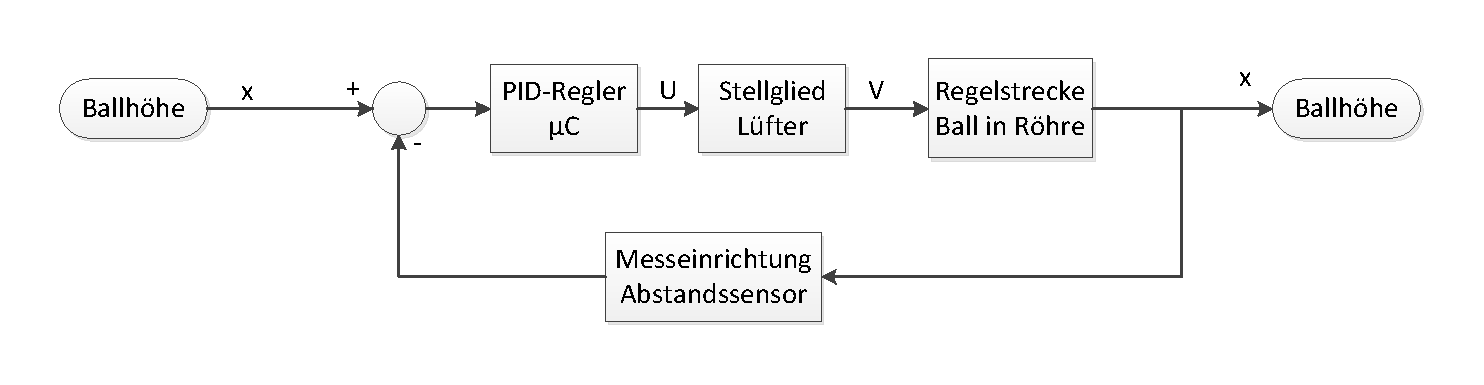
\includegraphics[width = \textwidth]{./Bilder/Blockschaltbild}
\caption{Blockschaltbild des Systems}
\label{pic:blockschaltbild}%
\end{figure}

%
%--------------------------------------------------------------------
%
%Teilaufgabe 2
%
\section{}\label{sec:einsinnvolleslabel1}
%

%
%Alle bisherigen Bilder einf�gen und einen Seitenumbruch erzwingen
\clearpage
